% =============================================================================
%  Subsubsection: End-to-End Off-Chain Identity / Credential Presentation
%                 Latency comparison of OIDC-Only, Private-key DID/VC,
%                 ZK-based VC, and zkDIDProof.
%
%  Drop-in for the experiment section of the zkEHR paper.
%
%  Required preamble (in the main paper):
%    \usepackage{booktabs}
%    \usepackage{graphicx}
%    \usepackage{amsmath}
%
%  Required figure file (next to this .tex, or anywhere on \graphicspath):
%    presentation-latency-comparison.pdf  (produced by make_figure.py)
% =============================================================================

\subsubsection{End-to-End Off-Chain Identity / Credential Presentation Latency}
\label{ssub:presentation-latency}

We compare the end-to-end presentation latency of \textsf{zkDIDProof} against
three baselines that span the design space of patient identity at a hospital
relying party: \textsf{OIDC-Only} (federated login, no decentralised identity),
\textsf{Private-key DID/VC} (a conventional self-sovereign DID with on-chain
registry), and \textsf{ZK-based VC} (the same DID/VC stack augmented with a
Groth16 selective-disclosure proof). All four schemes are exercised on the
same uniform message flow: hospital issues a fresh challenge $\to$ patient
acquires the identity material it will present $\to$ patient produces the
proof of possession $\to$ relying party verifies $\to$ a local patient
session is created. To make the credential-acquisition step
apples-to-apples, all VC-bearing schemes use a realistic OpenID4VCI flow:
the patient authenticates to the issuer via Google OIDC silent SSO, then
fetches the signed credential over HTTP from a co-located mock issuer that
verifies the patient's Google ID token before issuing.

\paragraph{Setup.}
All experiments run on an Ubuntu 24.04 \texttt{c5.large} EC2 instance in
\textit{us-east-1}, a single-vCPU configuration that mirrors the worst case
for serial cryptographic work. Each scheme executes 10 warm-up iterations
followed by 100 measured iterations of its full presentation flow; we report
the mean, median (p50), 95th- and 99th-percentile, and standard deviation of
the per-run end-to-end latency. Timings use Node.js
\texttt{process.hrtime.bigint()} (nanosecond resolution) and are reset between
runs. Schemes that require an OIDC ID token use a primed Chromium profile so
the silent-SSO path against Google reflects the realistic case of an
already-authenticated clinician browser. Schemes that require an on-chain
DID-object resolution point the Sui RPC client at the public Sui devnet
fullnode (also located in \textit{us-east-1}) and preserve HTTP/2 keepalive
across runs. One-time setup costs (DID-object registration on chain,
Groth16 trusted-setup, Chromium profile priming) are explicitly excluded
from the per-presentation budget; they are amortised in any deployed system.

\paragraph{Schemes.}
\textsf{OIDC-Only} measures the standard federated-login lower bound:
hospital nonce, Google ID token, JWT signature and claim validation, then
session. \textsf{Private-key DID/VC} models a conventional self-sovereign
stack: the patient holds a long-term Ed25519 key, registers a DID object on
Sui devnet (one-time), authenticates to a trusted clinic CA via Google
OIDC, fetches an Ed25519-signed verifiable credential, signs a fresh
hospital challenge, and presents the VC together with the signature; the
hospital resolves the on-chain DID object and verifies both the challenge
signature and the VC. \textsf{ZK-based VC} extends the prior flow with a
Groth16 selective-disclosure proof over the VC's claims that the patient
generates per presentation and the hospital verifies in addition to the
on-chain DID lookup. \textsf{zkDIDProof} (this paper) binds the hospital
challenge into the OIDC nonce via $\mathrm{nonce}_{\mathrm{jwt}} =
\mathrm{Poseidon}(r,\,T_{\mathrm{exp}},\,\mathrm{chal})$, has the patient
fetch a fresh Google ID token bearing that nonce, and produces a Groth16
proof attesting jointly to JWT validity, OIDC-derived DID derivation
($\mathrm{DID} = \mathrm{Poseidon}(\mathrm{sub},\,\mathrm{iss},\,
\mathrm{salt})$), challenge binding, and audience binding. The hospital
verifies the proof in-process against the verification key, with no
blockchain dependency at presentation time.

\paragraph{Cost regimes.}
Verifiable credentials are typically obtained once and reused across many
presentations (typical \texttt{exp}~$=$~weeks to months). To capture the two
operational extremes, we report results in two regimes:
(i)~the \emph{cold-start} regime, in which every presentation includes a
fresh credential acquisition (Google OIDC round-trip plus issuer HTTP
round-trip), and (ii)~the \emph{steady-state} regime, in which a previously
issued credential is reused, so the per-presentation budget excludes
\texttt{vc\_acquire\_oidc\_ms} and \texttt{vc\_acquire\_issuer\_rt\_ms}.
The two ZK-bearing schemes amortise their issuance cost in steady state;
\textsf{zkDIDProof}'s cost does not change between regimes because its
OIDC nonce binds the per-presentation challenge---the JWT cannot be cached
without breaking the challenge--response chain. \textsf{OIDC-Only} is
likewise unchanged across regimes because its ID token plays the same
role.

\paragraph{Results.}
Table~\ref{tab:presentation-latency-stats} and
Figure~\ref{fig:presentation-latency-comparison} summarise the four schemes
across both regimes. In the cold-start regime,
\textsf{Private-key DID/VC} (mean $277.1\,\mathrm{ms}$) and
\textsf{OIDC-Only} (mean $250.9\,\mathrm{ms}$) are clustered around the
$\approx 250\,\mathrm{ms}$ Google round-trip floor, while
\textsf{ZK-based VC} ($1364.7\,\mathrm{ms}$) and \textsf{zkDIDProof}
($1346.6\,\mathrm{ms}$) are clustered around the $\approx 1.0\,\mathrm{s}$
Groth16 proving floor; within each cluster the schemes are within $\sim 30\,\mathrm{ms}$
of one another. In the steady-state regime, however, the picture shifts
sharply: \textsf{Private-key DID/VC} drops to mean $21.5\,\mathrm{ms}$ and
\textsf{ZK-based VC} drops to mean $1074.3\,\mathrm{ms}$, while
\textsf{zkDIDProof} and \textsf{OIDC-Only} are unchanged.

The \emph{hospital-side} column tells the operationally relevant story.
\textsf{zkDIDProof} completes verification in $28.2\,\mathrm{ms}$
\emph{with no blockchain dependency} (Groth16 verify against a static
verification key, in-process), whereas \textsf{Private-key DID/VC} and
\textsf{ZK-based VC} pay $17.6\,\mathrm{ms}$ and $48.0\,\mathrm{ms}$
respectively, both \emph{requiring} a per-presentation Sui-RPC call. The
patient absorbs \textsf{zkDIDProof}'s $\approx 1.3\,\mathrm{s}$ proving cost
asymmetrically; relying-party scalability and offline operation are
determined by the hospital column. Across all four schemes, every measured
run succeeded and the coefficient of variation stays below~$3\%$ in both
regimes, so the means are representative and the percentile gaps are tight.

\paragraph{Trade-off.}
The four schemes occupy different points on a single trade-off curve.
\textsf{OIDC-Only} minimises end-to-end latency for federated logins but
provides no decentralised identity, no holder unlinkability, and no key
recoverability. \textsf{Private-key DID/VC} adds decentralised identity at
the price of a per-presentation chain fetch, exposes a long-term private
key, and---if the credential expires or is revoked---a fresh OIDC4VCI
issuance round costing $\approx 256\,\mathrm{ms}$. \textsf{ZK-based VC}
adds selective disclosure but pays \emph{both} a chain fetch and a Groth16
proof per presentation. \textsf{zkDIDProof} trades a $\approx 1.0\,\mathrm{s}$
patient-side proving cost for two structural gains the others cannot
match: (i)~the relying party verifies the proof in $\approx 28\,\mathrm{ms}$
with no blockchain dependency, and (ii)~the DID is bound to the patient's
OIDC subject through a hidden salt rather than a long-term key, enabling
keyless recovery and authority-blind unlinkability. Critically,
\textsf{zkDIDProof}'s number is invariant across the cold/steady regimes:
because the OIDC nonce binds the per-presentation challenge, the JWT cannot
be cached without breaking the challenge--response chain, so the
$\approx 1.3\,\mathrm{s}$ figure is the \emph{only} number---the scheme
admits no cache attack surface and no replay surface.
The qualitative consequences---offline verifiability, post-compromise
recovery, and unlinkability---are discussed in
Section~\ref{ssub:security-properties}.

% -----------------------------------------------------------------------------
% Statistical summary table — cold-start vs steady-state regimes.
% -----------------------------------------------------------------------------
\begin{table}[t]
  \centering
  \small
  \setlength{\tabcolsep}{4pt}
  \caption{End-to-end off-chain identity / credential presentation latency
    across the four schemes, in two regimes. \emph{Cold-start} includes a
    fresh credential-acquisition round on every presentation; \emph{steady-state}
    assumes the credential is cached and reused. All values are milliseconds
    over $n=100$ successful measured runs (warm-up $=10$, dropped) on
    \texttt{c5.large} (\textit{us-east-1}). Lower is better.
    \textsf{zkDIDProof} and \textsf{OIDC-Only} are invariant across regimes
    by design.}
  \label{tab:presentation-latency-stats}
  \begin{tabular}{lrrrrr|rrrrr}
    \toprule
    & \multicolumn{5}{c|}{Cold-start} & \multicolumn{5}{c}{Steady-state} \\
    Scheme & Mean & p50 & p95 & p99 & Std. & Mean & p50 & p95 & p99 & Std. \\
    \midrule
    OIDC-Only             & $250.93$  & $242.54$  & $324.77$  & $393.85$  & $34.52$  & $250.93$  & $242.54$  & $324.77$  & $393.85$  & $34.52$ \\
    Private-key DID/VC    & $277.07$  & $275.25$  & $321.76$  & $421.78$  & $26.61$  & $\phantom{0}21.46$   & $\phantom{0}15.60$   & $\phantom{0}58.39$   & $149.50$  & $18.16$ \\
    ZK-based VC           & $1364.69$ & $1360.76$ & $1395.41$ & $1521.81$ & $24.96$  & $1074.29$ & $1069.60$ & $1120.57$ & $1238.74$ & $22.67$ \\
    \textbf{zkDIDProof (ours)} & $\mathbf{1346.56}$ & $\mathbf{1343.24}$ & $\mathbf{1384.09}$ & $\mathbf{1544.56}$ & $\mathbf{26.19}$ & $\mathbf{1346.56}$ & $\mathbf{1343.24}$ & $\mathbf{1384.09}$ & $\mathbf{1544.56}$ & $\mathbf{26.19}$ \\
    \bottomrule
  \end{tabular}
\end{table}

% -----------------------------------------------------------------------------
% Patient-side vs hospital-side cost figure (two-panel: cold + steady).
% -----------------------------------------------------------------------------
\begin{figure}[t]
  \centering
  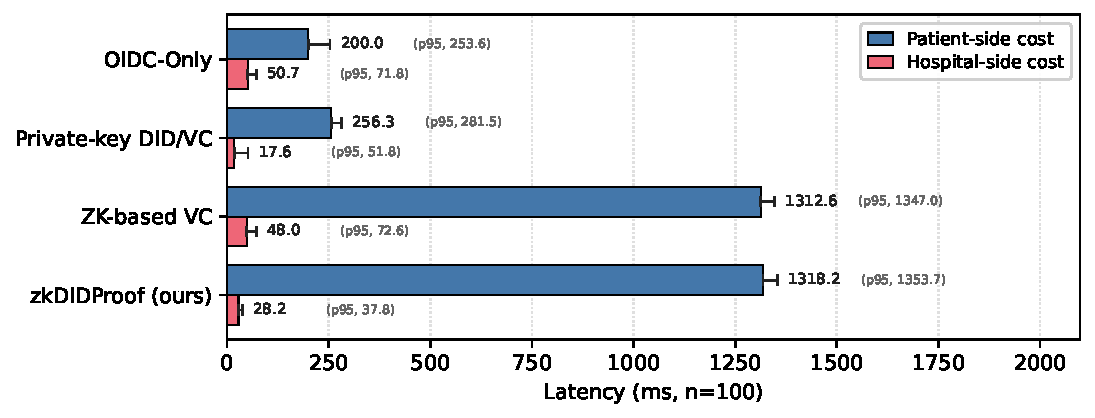
\includegraphics[width=\textwidth]{presentation-latency-comparison}
  \caption{End-to-end off-chain presentation latency by scheme, decomposed
    into \emph{patient-side} cost (work performed to produce the
    presentation) and \emph{hospital-side} cost (work performed by the
    relying party to verify and create a session). Bars show the mean over
    $n=100$ successful runs; the $x$-axis is logarithmic in both panels.
    Panel~(a) is the \emph{cold-start} regime, in which every presentation
    includes a fresh credential acquisition (Google OIDC round-trip plus
    issuer HTTP round-trip). Panel~(b) is the \emph{steady-state} regime,
    in which the credential is cached and reused. Hospital-side cost
    includes a Sui-devnet RPC fetch for the chain-anchored schemes
    (\textsf{Private-key DID/VC}, \textsf{ZK-based VC});
    \textsf{zkDIDProof} contains no chain dependency at presentation time
    and is invariant across regimes because its per-presentation OIDC nonce
    binds the hospital challenge.}
  \label{fig:presentation-latency-comparison}
\end{figure}
